\documentclass[UTF8, a4paper, zihao=-4, bibliography=totoc]{ctexart}
\usepackage{color}
\usepackage[dvipsnames]{xcolor}
\usepackage{mathtools}
\usepackage[colorlinks=true, pdfstartview=FitH, linkcolor=black, anchorcolor=violet, citecolor=magenta]{hyperref}
\usepackage{graphicx}
\usepackage{enumitem}
\usepackage{titlesec}
\usepackage{titletoc}
\usepackage{bm}
\usepackage{amsmath}
\usepackage{amsfonts}
\usepackage{mathrsfs}
\usepackage{multirow}
\usepackage{amsthm}
\usepackage{tabularx, booktabs}
\usepackage{longtable}
\usepackage{supertabular}
\usepackage{array, makecell}
\usepackage{graphicx}
\usepackage{epstopdf}
\usepackage{float}
\usepackage{subfigure}
\usepackage{geometry}
\usepackage{ctex}
\usepackage{listings}
\usepackage[nottoc,numbib]{tocbibind}
\usepackage[backend=biber, style=gb7714-2015]{biblatex}
\addbibresource[location=local]{../reference.bib}
\usepackage{pythonhighlight}
\usepackage{caption}
\usepackage{booktabs}
\usepackage{algorithm}
\usepackage{algorithmic}
\usepackage[toc]{appendix}
\usepackage{xhfill}
%%%%%%%%%%%%%%%%%%%%%%%%%%%%%%%%%%%%%%%%%%%%%%%%%%%%%%%%%%%%%%%%%%%%%%%%%%%%%%%%
%%%%%%%%%%%%%%%%%%%%%%%%%%%%%%%%% ctexset %%%%%%%%%%%%%%%%%%%%%%%%%%%%%%%%%%%%%%
%%%%%%%%%%%%%%%%%%%%%%%%%%%%%%%%%%%%%%%%%%%%%%%%%%%%%%%%%%%%%%%%%%%%%%%%%%%%%%%%
\ctexset{
    bibname     =   {参考文献},
    section = {
        number  =   \arabic{section},
        format  +=  \zihao{-4}\raggedright,
        name    =   {,.},
    },
    subsection = {
        format  =  \bf{\zihao{-4}}\raggedright,
    },
    subsubsection = {
        number  =   \arabic{subsubsection},
        format  +=  {\zihao{-4}}\raggedright,
    }
}

% 用来设置附录中代码的样式

\definecolor{mygreen}{RGB}{28,172,0} % color values Red, Green, Blue
\definecolor{mylilas}{RGB}{170,55,241}

\lstset{
    basicstyle          =   \sffamily,
    keywordstyle        =   \bfseries,
    commentstyle        =   \rmfamily\itshape,
    stringstyle         =   \ttfamily,
    flexiblecolumns,
    numbers             =   left,
    showspaces          =   false,
    numberstyle         =   \zihao{-5}\ttfamily,
    showstringspaces    =   false,
    captionpos          =   t,
    frame               =   lrtb,
}

\lstdefinestyle{Python}{
    language        =   Python,
    basicstyle      =   \zihao{-5}\ttfamily,
    numberstyle     =   \zihao{-5}\ttfamily,
    keywordstyle    =   \color{blue},
    keywordstyle    =   [2] \color{teal}, % just to check that it works
    stringstyle     =   \color{magenta},
    commentstyle    =   \color{mygreen}\ttfamily,
    breaklines      =   true,
    columns         =   fixed,
    basewidth       =   0.5em,
}

\lstdefinestyle{MATLAB}{
    language        =   Matlab,
    basicstyle      =   \zihao{-5}\ttfamily,
    numberstyle     =   \zihao{-5}\ttfamily,
    keywordstyle    =   \color{blue},
    keywordstyle    =   [2] \color{teal}, % just to check that it works
    stringstyle     =   \color{mylilas},
    commentstyle    =   \color{mygreen}\ttfamily,
    breaklines      =   true,
    columns         =   fixed,
    basewidth       =   0.5em,
}

\theoremstyle{definition}

\newtheorem{definition}{定义}[section]

\newtheorem{theorem}{定理}[section]

\newtheorem{corollary}{推论}[theorem]

\newtheorem{lemma}[theorem]{引理}

\newenvironment{myquote}
    {\begin{quote}\kaishu\zihao{5}}
    {\end{quote}}

\setcounter{MaxMatrixCols}{20}

\renewcommand{\algorithmicrequire}{ \textbf{Input:}} %Use Input in the format of Algorithm 
\renewcommand{\algorithmicensure}{ \textbf{Output:}} %UseOutput in the format of Algorithm
% 定义页面边距

\newgeometry{
    left=2.5cm,
    right=2.0cm,
    top=2.5cm,
    bottom=2.5cm
}

\newcommand{\ThisProjectTitle}{插值法}
\newcommand{\ThisDate}{2017年11月29日}
\newcommand{\ThisNo}{No.3}

%%%%%%%%%%%%%%%%%%%%%%%%%%%%%%%%%%%%%%%%%%%%%%%%%%%%%%%%%%%%%%%%%%%%%%%%%%%%%%%%
%%%%%%%%%%%%%%%%%%%%%%%%%%%%%%%%%%% document %%%%%%%%%%%%%%%%%%%%%%%%%%%%%%%%%%%
%%%%%%%%%%%%%%%%%%%%%%%%%%%%%%%%%%%%%%%%%%%%%%%%%%%%%%%%%%%%%%%%%%%%%%%%%%%%%%%%

\begin{document}

\newcommand{\CourseName}{{\bf 课程名称:}}
\newcommand{\Grade}{{\bf 年级:}}
\newcommand{\Score}{{\bf 上机实践成绩:}}
\newcommand{\Director}{{\bf 指导教师:}}
\newcommand{\StudentName}{{\bf 学生姓名:}}
\newcommand{\ProjectTitle}{{\bf 上机实践名称:}}
\newcommand{\StudentID}{{\bf 学号:}}
\newcommand{\Date}{{\bf 上机实践日期:}}
\newcommand{\No}{{\bf 上机实践编号:}}
\newcommand{\GroupNum}{{\bf 组号:}}
\newcommand{\LastEditTine}{{\bf 最后修改时间:}}

\newcommand{\ThisCourseName}{数值计算实验}
\newcommand{\MyGrade}{2015级}
\newcommand{\MyScore}{100}
\newcommand{\MyDirector}{朱娟萍}
\newcommand{\MyName}{刘鹏}
\newcommand{\ThisProjectTitle}{非线性方程求根}
\newcommand{\MyID}{20151910042}
\newcommand{\ThisDate}{2017-10-16}
\newcommand{\ThisNo}{No.1}
\newcommand{\MyGroupNum}{1}
\newcommand{\MyLastEditTine}{\today}

\newcommand{\HRule}{\rule{\linewidth}{0.3mm}}
\newcommand{\xfill}[2][1ex]{{%
  \dimen0=#2\advance\dimen0 by #1
  \leaders\hrule height \dimen0 depth -#1\hfill%
}}
\newcommand{\xfilll}[2][1ex]{%
  \dimen0=#2\advance\dimen0 by #1%
  \leaders\hrule height \dimen0 depth -#1\hfill%
}

\begin{center}
    {\zihao{3} \bf 云南大学数学与统计学院}\\
    {\zihao{3} \bf 上机实践报告}
\end{center}

\begin{table}[h]
    \centering
    \resizebox{\textwidth}{!}{%
        \begin{tabular}{|l|l|l|}
        \hline
            \CourseName \ThisCourseName     & \Grade \MyGrade       & \Score                        \\ \hline
            \Director \MyDirector           & \StudentName \MyName  &                               \\ \hline
            \ProjectTitle \ThisProjectTitle & \StudentID \MyID      & \Date \ThisDate               \\ \hline
            \No \ThisNo                     & \GroupNum             & \LastEditTine \MyLastEditTine \\ \hline
        \end{tabular}
    }
    \xfill{30pt}
\end{table}

\section{实验目的}

1. 通过对所学的线性方程组直接求解的理论方法进行编程,提升程序编写水平;

2. 通过对理论方法的编程实验,进一步掌握理论方法的每一个细节;

3. 通过数值法求解,发现数值方法与符号方法的区别,并形成专业思维。

\section{实验内容}

1. 编程实现高斯-若尔当列主元消元法;

2. 编程实现高斯-若尔当全主元消元法;

3. 任选一种方案,Doolittle分解或者Crout分解,编程实现矩阵的LU分解;

4. 编程实现三对角线矩阵的稀疏方式存储,然后对其进行LU分解。

\section{实验平台}

macOS

Python 3.7.3;

MATLAB R2017b win64;

\section{实验记录与实验结果分析}

\subsection{第1题}

1题
编程实现:用高斯-若尔当列主元消元法求下列方程的解[1]:

\begin{equation}
    \left\{\begin{aligned}
        x_{1}+2 x_{2}+x_{3}     &=  2   \\
        -2 x_{1}-2 x_{2}-x_{3}  &=  -3  \\
        2 x_{1}-3 x_{2}-2 x_{3} &=  -1 
    \end{aligned}\right.
\end{equation}

\subsubsection{程序代码}

\lstinputlisting[
    style       =   Python,
    %caption     =   {\bf ff.py},
    label       =   {get_root.py}
]{../../src/3_线性方程组的直接解法/ColumnPivotMethod.py}

\subsubsection{运行结果}

\subsubsection{结果分析}

由于二分法与埃特金方法的函数并不是一样的,前者是原函数,后者是迭代函数,所以很难写一个通用算法解决这个迭代函数的生成问题。所以这个class意义不是很大,不过可以通过对属性进行赋值,重复进行计算,也算有一定的灵活性。

\section{实验体会}

通过编程,复习了简单迭代法及其改进。明白了二分法与埃特金法的斯坦弗森过程之间的区别。

\section{参考文献}

[1] 金一庆, 陈越, 王冬梅. 数值方法[M]. 北京: 机械工业出版社; 2000.2.


\section{实验目的}
\begin{enumerate}[leftmargin=1.4cm, itemsep=-0.5mm]
    \item 通过对所学的插值法的理论方法进行编程,提升程序编写水平;
    \item 通过对理论方法的编程实验,进一步掌握理论方法的每一个细节;
    \item 检验教材知识的理解与掌握程度。
\end{enumerate}

\section{实验内容}
\begin{enumerate}[leftmargin=1.4cm, itemsep=-0.5mm]
    \item 编制用拉格朗日插值方法进行插值的程序;
    \item 编制用牛顿插值方法进行插值的程序;
    \item 要求牛顿插值方法在等距与不等距下两种情况下,程序可以进行自行选择,降低计算量。
\end{enumerate}

\section{实验平台}
macOS

Python 3.7.3

MATLAB R2019a

\section{实验记录与实验结果分析}

\subsection{第1题}
\begin{quote}
    {\kaishu
        已知正弦函数表:
        \begin{table}[H]
            \centering
            \begin{tabular}{@{}lllllllll@{}}
            \toprule
                $x_k$ & 0.5 & 0.7 & 0.9 & 1.1 & 1.3 & 1.5 & 1.7 & 1.9 \\ \midrule
                $\sin(x_k)$ & 0.4794 & 0.6442 & 0.7833 & 0.8912 & 0.9636 & 0.9975 & 0.9917 & 0.9463\\ \bottomrule
            \end{tabular}%
        \end{table}
        编写程序,分别用拉格朗日插值和牛顿插值多项式计算$x_0=0.6,\ 0.8,\ 1.0$处的函数值$\sin(0.6)$,$\sin(0.8)$,$\sin(1.0)$的近似值$f(0.6)$,$f(0.8)$,$f(1.0)$
    }
\end{quote}

程序代码参见\ref{1-Interpolation-Methods.py}
\subsubsection{运行结果}

\begin{lstlisting}[style = bash]
$ python3 1-Interpolation-Methods.py 
+----------+---------+--------------+
|  Method  |    x    |       y      |
+----------+---------+--------------+
|   Lagr   |   0.6   |    0.5646    |
|          |   0.8   |    0.7173    |
|          |   1.0   |    0.8414    |
+----------+---------+--------------+
|  Newton  |   0.6   |    0.5624    |
|          |   0.8   |    0.7181    |
|          |   1.0   |    0.8402    |
+----------+---------+--------------+
\end{lstlisting}

\begin{figure}[H]
    \centering
    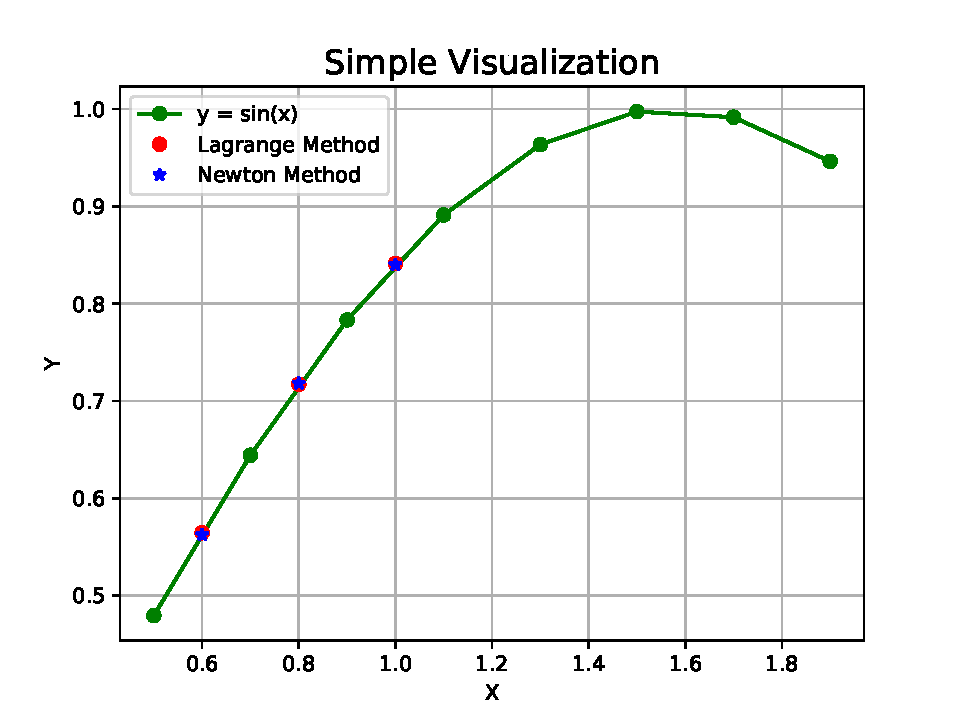
\includegraphics[width=0.7\textwidth]{../../img/06/lagrange.pdf}
    \caption{拉格朗日插值}
    \label{Fig:Lagrange}
\end{figure}

\subsubsection{结果分析}

本段代码,是构建了一个简单的封装,可以将已知点作为参数输入,然后输入作为第三个参数的要估计的点的横坐标列表,最终返回一个列表,它储存着根据相应方法得到的插值数值。

%%%%%%%%%%%%%%%%%%%%%%%%%%%%%%%%%%%%%%%%%%%%%%%%%%%%%%%%%%%%%%%%%%%%%%%%%%%%%%%%
%%%%%%%%%%%%%%%%%%%%%%%%%%%%%%%%%%% PROBLEM %%%%%%%%%%%%%%%%%%%%%%%%%%%%%%%%%%%%
%%%%%%%%%%%%%%%%%%%%%%%%%%%%%%%%%%%%%%%%%%%%%%%%%%%%%%%%%%%%%%%%%%%%%%%%%%%%%%%%

\subsection{第2题}
\begin{quote}
    {\kaishu
        已知
        \begin{table}[H]
            \centering
            \begin{tabular}{@{}lllllllll@{}}
            \toprule
                $x$ & 0.4 & 0.5 & 0.6 & 0.7 & 0.8 & 0.9 \\ \midrule
                $\ln(x_k)$ & $-0.916\ 291$ & $-0.693\ 147$ & $-0.510\ 826$ & $-0.357\ 765$ & $-0.223\ 144$ & $-0.105\ 361$\\ \bottomrule
            \end{tabular}%
        \end{table}
        用牛顿后插公式求$\ln⁡(0.78)$的近似值,并根据5阶差分估计4阶公式的误差。
    }
\end{quote}

程序代码参见\ref{2-Newton-left-interp-Method.py}

\subsubsection{运行结果}

\begin{lstlisting}[style = bash]
$ python3 2-Newton-left-interp-Method.py 
-0.24887097759999988
-0.2484613592984996
+----------+----------+---------------+
|  Method  |    x     |       y       |
+----------+----------+---------------+
|   Lagr   |   0.41   |    -0.8919    |
|          |   0.51   |    -0.6732    |
|          |   0.61   |    -0.4944    |
|          |   0.71   |    -0.3436    |
|          |   0.81   |    -0.2105    |
|          |   0.89   |    -0.1161    |
+----------+----------+---------------+
|  Newton  |   0.41   |    -0.8919    |
|          |   0.51   |    -0.6732    |
|          |   0.61   |    -0.4944    |
|          |   0.71   |    -0.3436    |
|          |   0.81   |    -0.2105    |
|          |   0.89   |    -0.1161    |
+----------+----------+---------------+
\end{lstlisting}

\begin{figure}[H]
    \centering
    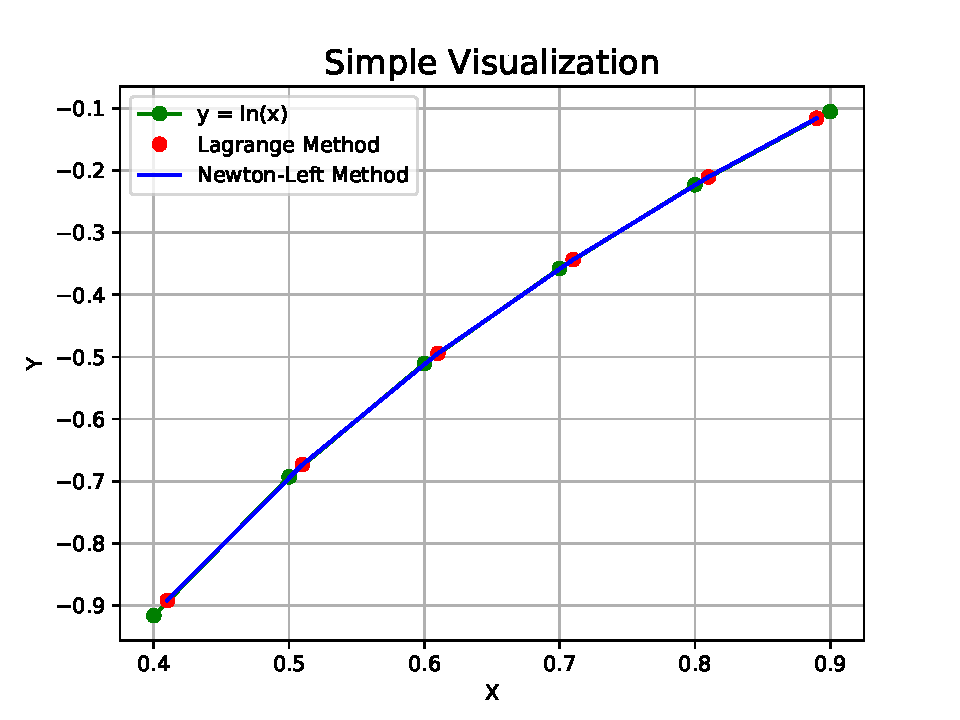
\includegraphics[width=0.7\textwidth]{../../img/06/newton.pdf}
    \caption{牛顿插值}
    \label{Fig:newton}
\end{figure}

\subsubsection{结果分析}
牛顿后插公式,就是在等距节点的基础上,简化了差商的计算,但是需要计算一个独立的差分表。差分表的构建需要依据前插还是后插,其中前插表得到的是一个上三角矩阵,后插公式得到的是一个下三角矩阵。得到了差分表,就可以根据对角线元素,构建差商表。然后根据题目1的已有代码,即可做出图像。

\section{实验体会}

本次实验难度较小,代码量不算大。

之前想过用MATLAB做03号实验,但是后来还是决定继续采用Python3,首先是平台比较开放,其次是本次基本不涉及矩阵,就算是涉及到矩阵运算,也已经有了一个由我独立设计的比较完善的Python包,所以坚持Python可能是一个比较好的选择。

插值算法的核心在于解方程组。而在牛顿插值多项式中,引入差商概念,用差商推导出了一般的插值计算公式,同时给出了很明确的算法与误差估计。其形式与泰勒展开式非常相似,余项也和泰勒公式非常像。

\section{参考文献}

\printbibliography[heading=none]


\section{代码附录}
\label{附录}

\subsubsection{插值法}
\lstinputlisting[
    style       =   Python,
    caption     =   {\bf 1-Interpolation-Methods.py},
    label       =   {1-Interpolation-Methods.py}
]{../../src/6_插值法/1-Interpolation-Methods.py}

\subsection{条件数}
\lstinputlisting[
    style       =   Python,
    caption     =   {\bf 2-Newton-left-interp-Method.py},
    label       =   {2-Newton-left-interp-Method.py}
]{../../src/6_插值法/2-Newton-left-interp-Method.py}

\end{document}
